
\begin{center}
\LARGE
Matematikscreening (8:00 - 10:00)
\end{center}
\stepcounter{section}

\begin{opgavetekst}{Opgave 1}
En funktion $f$ er givet ved 
\begin{align*}
f(x) = 7x - 21.
\end{align*}
\end{opgavetekst}
\begin{delopgave}{(5 point)}{1}
		Bestem $f(-3)$.
\end{delopgave}
\begin{delopgave}{(5 point)}{2}
	Bestem skæringspunktet mellem grafen for $f$ og førsteaksen.
\end{delopgave}
\begin{opgavetekst}{Opgave 2}
	På Figur \ref{fig:lines} ses graferne for tre lineære funktioner $f$, $g$ og $h$ 
	med forskrifterne 
	\begin{align*}
		f(x) &= 2x-1,\\
		g(x) &= 4x,\\
		h(x) &= -x+5.
	\end{align*}
	Desuden ses punktet $P(2,y)$, der ligger på skæringen mellem graferne $A$ og $B$.
	\begin{figure}[H]
		\centering
		\begin{tikzpicture}
			\begin{axis}[
				axis lines = center,
				xmin = -3,
				ymin = -1
				]
				\addplot[samples = 10, color = green] {2*x-1};
				\addplot[samples = 10, color = red]	{4*x};
				\addplot[samples = 10, color = blue] {-x+5};
				
				\node at (axis cs:2,4) {$P$};
				\draw[dashed, color = gray, thick] (axis cs: 2,0 ) -- (axis cs:2,3);
				\draw[dashed, color = gray, thick] (axis cs: 0,3 ) -- (axis cs:2,3);
				\node at (axis cs:-0.23,3) {$y$};
				\node[color = blue] at (axis cs:-0.7,7) {$A$};
				\node[color = green] at (axis cs:4,5.5) {$B$};
				\node[color = red] at (axis cs:2,9.5) {$C$};
				\node[circle, fill = purple, inner sep = 0pt, minimum size = 5pt] at (axis cs: 2,3) {};
			\end{axis}
			\node at (9,0.3) {(1)};
			\node at (3.15,7.5) {(2)};
		\end{tikzpicture}
		\caption{Graferne for funktionerne $f$, $g$ og $h$.}
		\label{fig:lines}
	\end{figure}\phantom{h}
\end{opgavetekst}
\begin{delopgave}{(10 point)}{1}
	Afgør, hvilke af graferne $A$, $B$ og $C$, der tilhører funktionerne $f$, $g$ og $h$. 
\end{delopgave}
\begin{delopgave}{(5 point)}{2}
	Brug dit svar på a) til at bestemme andenkoordinaten $y$ i punktet $P(2,y)$.
\end{delopgave}

\begin{opgavetekst}{Opgave 3}
	En ligning er givet ved
	\begin{align*}
		2(x-4) = 5x+1.
	\end{align*}
\end{opgavetekst}
\begin{delopgave}{(10 point)}{1}
	Løs ligningen \textbf{uden} brug af \textit{solve}, hvor du argumenterer for, hvad du gør linje for linje.
\end{delopgave}
\begin{delopgave}{(5 point)}{2}
	Løs ligningen \textbf{med} brug af \textit{solve}, og undersøg om dit resultat passer med resultatet fra a).
\end{delopgave}

\begin{opgavetekst}{Opgave 4}
	På Figur \ref{fig:oneline} ses grafen for en lineær funktion $f$ givet ved
	\begin{align*}
		f(x) = ax + b.
	\end{align*}
	\begin{figure}[H]
		\centering
		\begin{tikzpicture}
			\begin{axis}[
				axis lines = center,
				xmin = -1,
				ymin = -5, 
				ticks = none
				]
				\addplot[samples = 10, color = blue!40, thick] {2*x-4};
				\node[circle, fill = purple, inner sep = 0pt, minimum size = 5pt] at (axis cs: 1,-2) {};
				\node[circle, fill = purple, inner sep = 0pt, minimum size = 5pt] at (axis cs: 3,2) {};
				\node at (axis cs:1.7,-2) {$P(1,-2)$};
				\node at (axis cs:3.7,2) {$Q(3,2)$};
				\node at (axis cs:4,5) {$\color{blue!60} f$};
			\end{axis}
			\node at (8.9,3.2) {(1)};
			\node at (1.4,7.5) {(2)};
		\end{tikzpicture}
		\caption{Grafen for $f$.}
		\label{fig:oneline}
	\end{figure}\phantom{h}
\end{opgavetekst}
\begin{delopgave}{(10 point)}{1}
	Brug punkterne på Figur \ref{fig:oneline} til at bestemme $a$ og $b$. 
\end{delopgave}
\begin{delopgave}{(5 point)}{2}
	Bestem forskriften for $f$ og brug denne til at bestemme $f(4)$. 
\end{delopgave}
\begin{delopgave}{(5 point)}{3}
	Løs ligningen $f(x) = 0$.
\end{delopgave}

\begin{opgavetekst}{Opgave 5}
	\begin{center}
	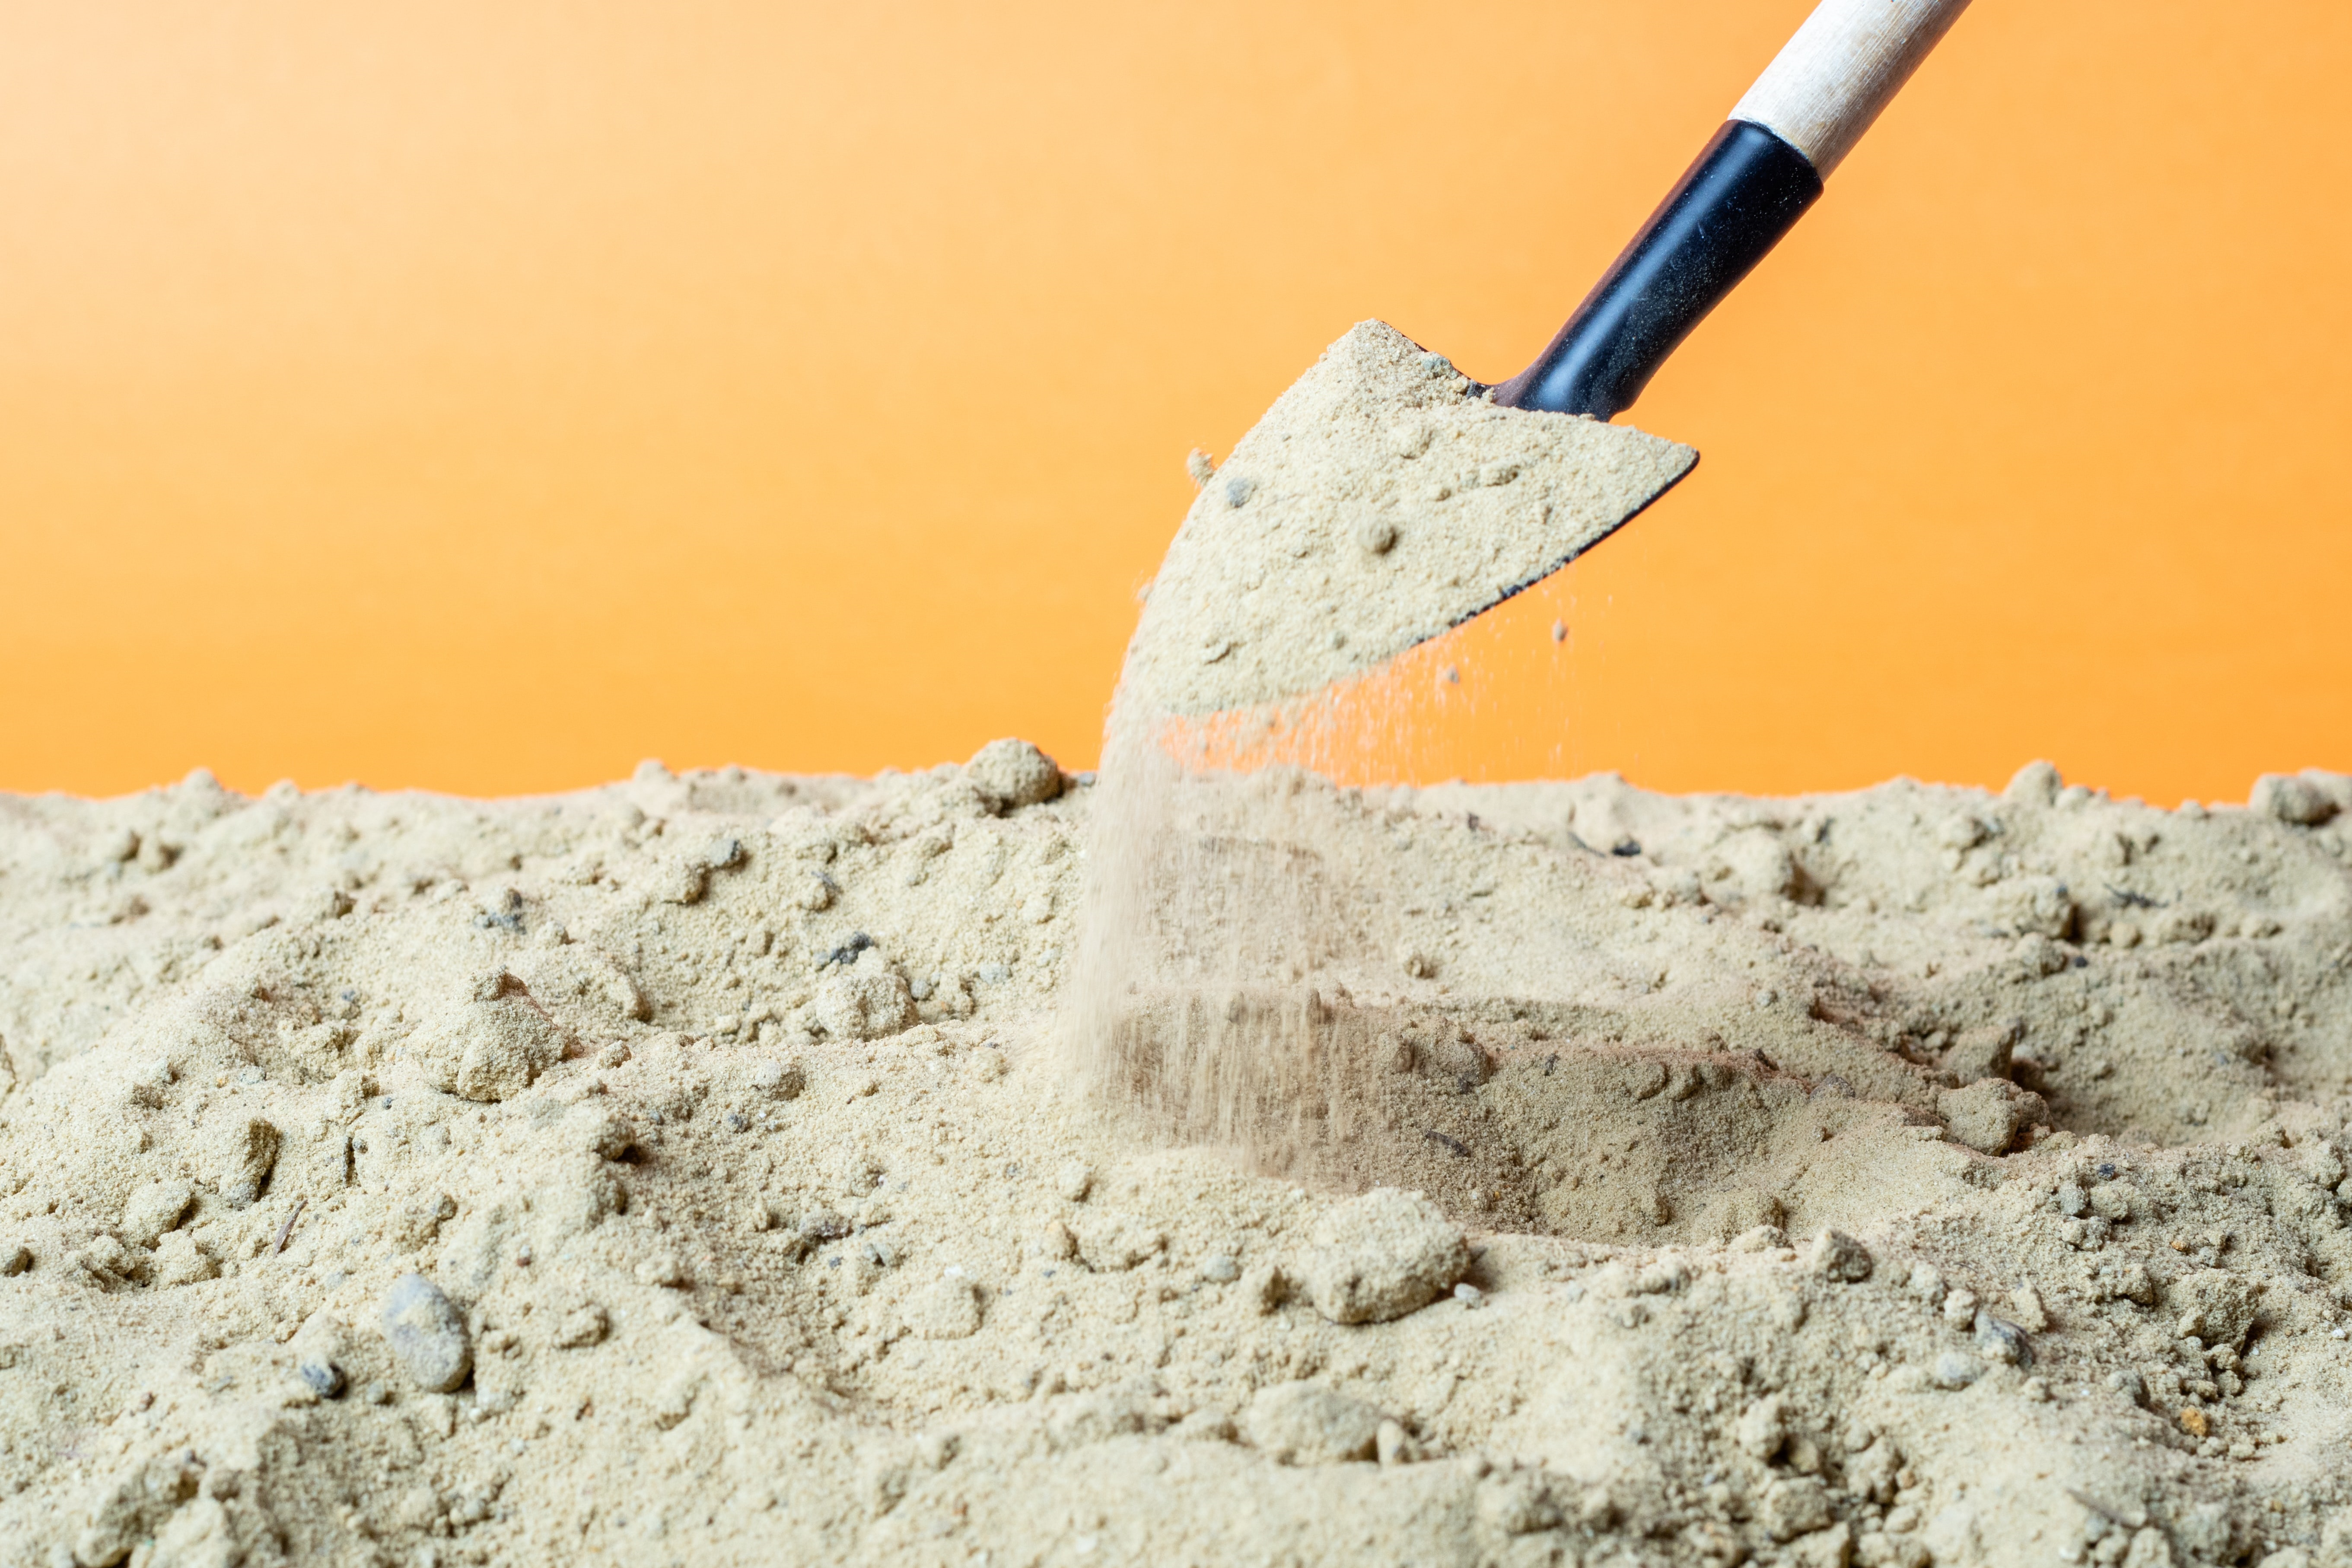
\includegraphics[width= 0.6\textwidth]{Billeder/sand.jpg}
	\end{center}
	En gruppe venner skovler sand til et byggeprojekt. Mængden af sand de kan skovle sammenholdt med antallet af personer kan ses af Tabel \ref{tab:sand}.
	
	\begin{table}[H]
		\centering
		\begin{tabular}{c|c|c|c|c|c}
		Personer & 1 & 2 & 3 & 4 & 5 \\
		\hline
		Sand (kg) per time  & 870 & 1700 & 2510 & 3490 & 4280	
		\end{tabular}
		\caption{Skovlet sand.}
		\label{tab:sand}
	\end{table}
	Vi antager, at mængden af skovlet sand $S$ (i kg per time) som funktion af antal personer $x$ kan beskrives ved sammenhængen
	\begin{align*}
		S(x) = ax+b.
	\end{align*}
\end{opgavetekst}
\begin{delopgave}{(10 point)}{1}
	Brug tallene fra Tabel \ref{tab:sand} til at bestemme $a$ og $b$. 
\end{delopgave}
\begin{delopgave}{(10 point)}{2}
	For at blive færdige i tide skal de kunne skovle 8000 kg sand i timen. Hvor mange personer skal de mindst være ifølge modellen for at nå dette?
\end{delopgave}

\begin{opgavetekst}{Opgave 6}
	På Figur \ref{fig:twolines} ses graferne for funktionerne $f$ og $g$ givet ved henholdsvist 
	\begin{align*}
		f(x) &= -x+5,\\
		g(x) &= 2x-1.	
	\end{align*}	 
	\begin{figure}[H]
		\centering
		\begin{tikzpicture}
			\begin{axis}[
				axis lines = center,
				xmin = -3,
				ymin = -1,
				ticks = none
				]
				\addplot[samples = 10, color = blue!40, thick] {2*x-1};
				\addplot[samples = 10, color = red!40, thick]	{-x+5};
				\node[circle, fill = purple, inner sep = 0pt, minimum size = 5pt] at (axis cs: 2,3) {};
				\node at (axis cs:2,4) {$P$};
				\node at (axis cs: 4.5,1.3) {$\color{red!60} f$};
				\node at (axis cs: 4.5,7.2) {$\color{blue!60} g$};
			\end{axis}
			\node at (9,0.7) {(1)};
			\node at (3.15,7.5) {(2)};
		\end{tikzpicture}
		\caption{Graferne for funktionerne $f$ og $g$.}
		\label{fig:twolines}
	\end{figure}\phantom{h}
\end{opgavetekst}
\begin{delopgave}{(10 point)}{1}
	Bestem koordinaterne til skæringspunktet $P$ mellem graferne for $f$ og $g$. 
\end{delopgave}

\begin{opgavetekst}{Opgave 7}
	\begin{center}
		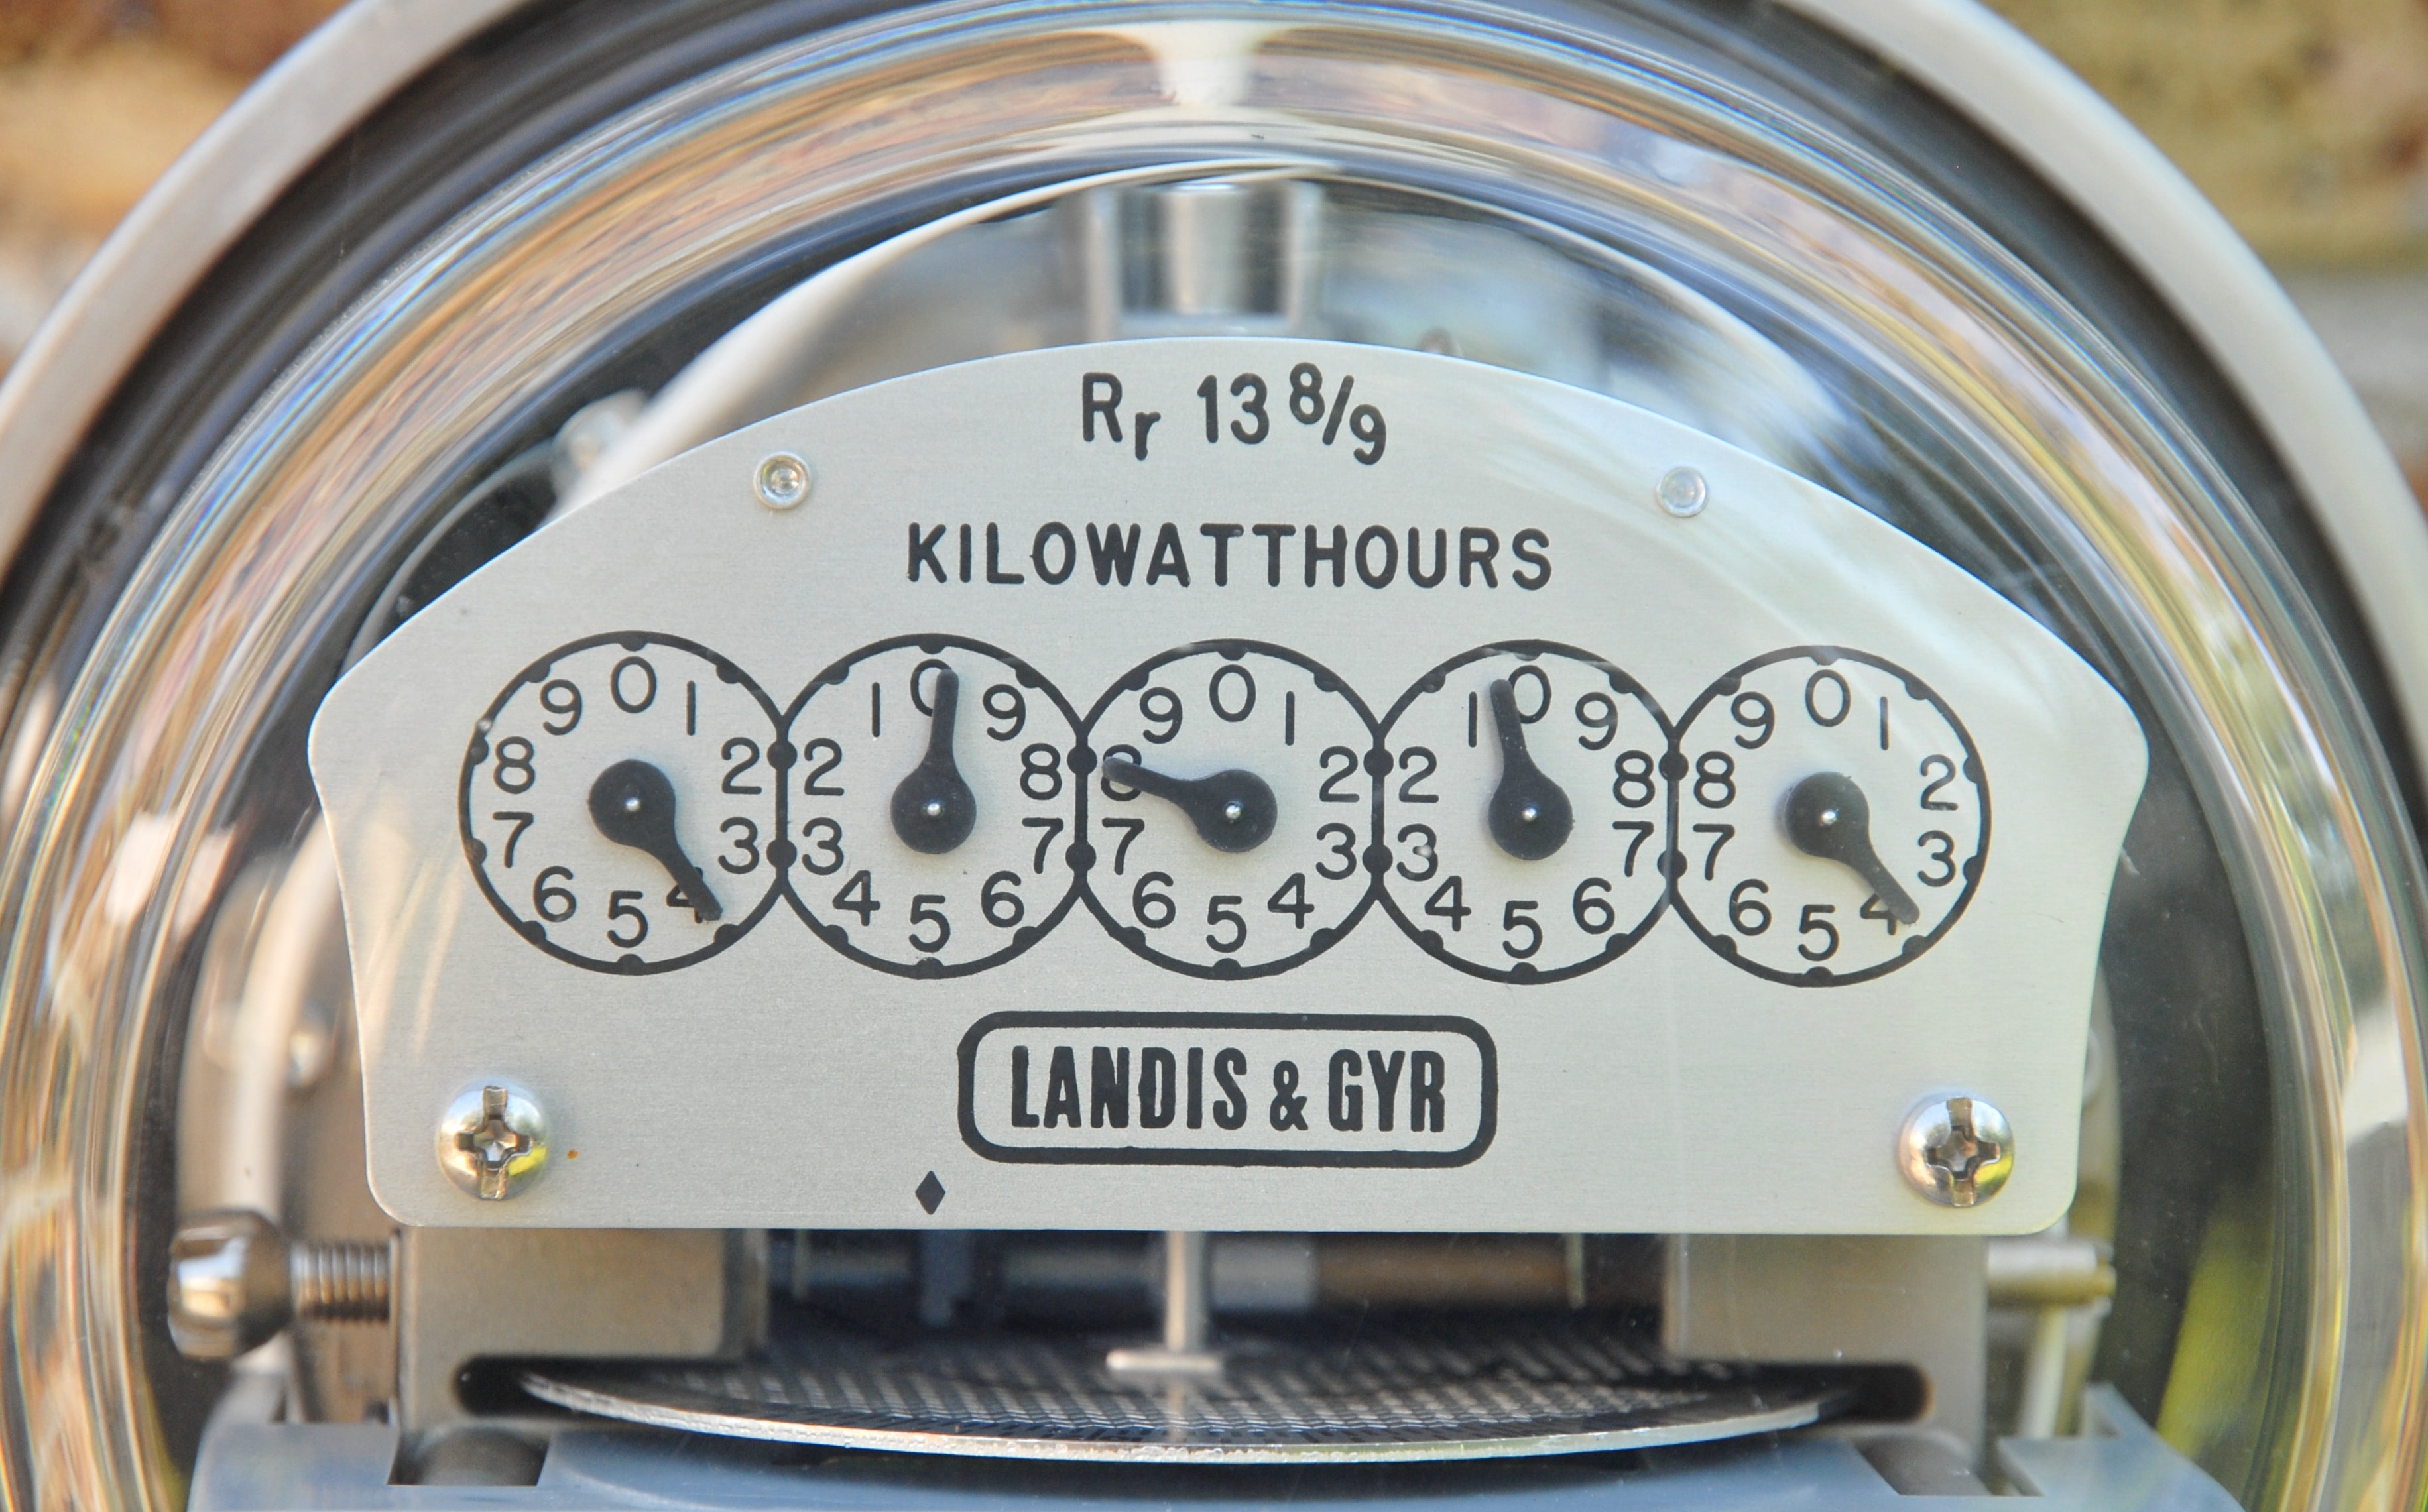
\includegraphics[width = 0.5\textwidth]{Billeder/el.jpg}
	\end{center}
	En person aflæser hver dag på sin elmåler og opdager, at den dagligt stiger med 7kWh. Da 
	han startede med at aflæse stod elmåleren på 33015kWh.
\end{opgavetekst}
\begin{delopgave}{(10 point)}{1}
	Indfør passende variable og opstil en model, der beskriver sammenhængen mellem den totale
	el, som er gennemløbet elmåleren og den forløbne tid. 
\end{delopgave}
